\chapter{Wybrane fragmenty implementacji}

\section{Przykład uruchomienia aplikacji i interpretacja wyników}

Aby uruchomić eksperymenty, należy skorzystać z polecenia \texttt{make pipeline}, które uruchamia główny potok eksperymentalny:
\begin{verbatim}
UV_CACHE_DIR=.cache/uv PYTHONPATH=src uv run python -m glopt.experiments.pipeline
\end{verbatim}

Na rysunku~\ref{fig:cli-content} przedstawiono przykładowy przebieg uruchomienia aplikacji z poziomu terminala.

\begin{figure}[H]
    \centering
    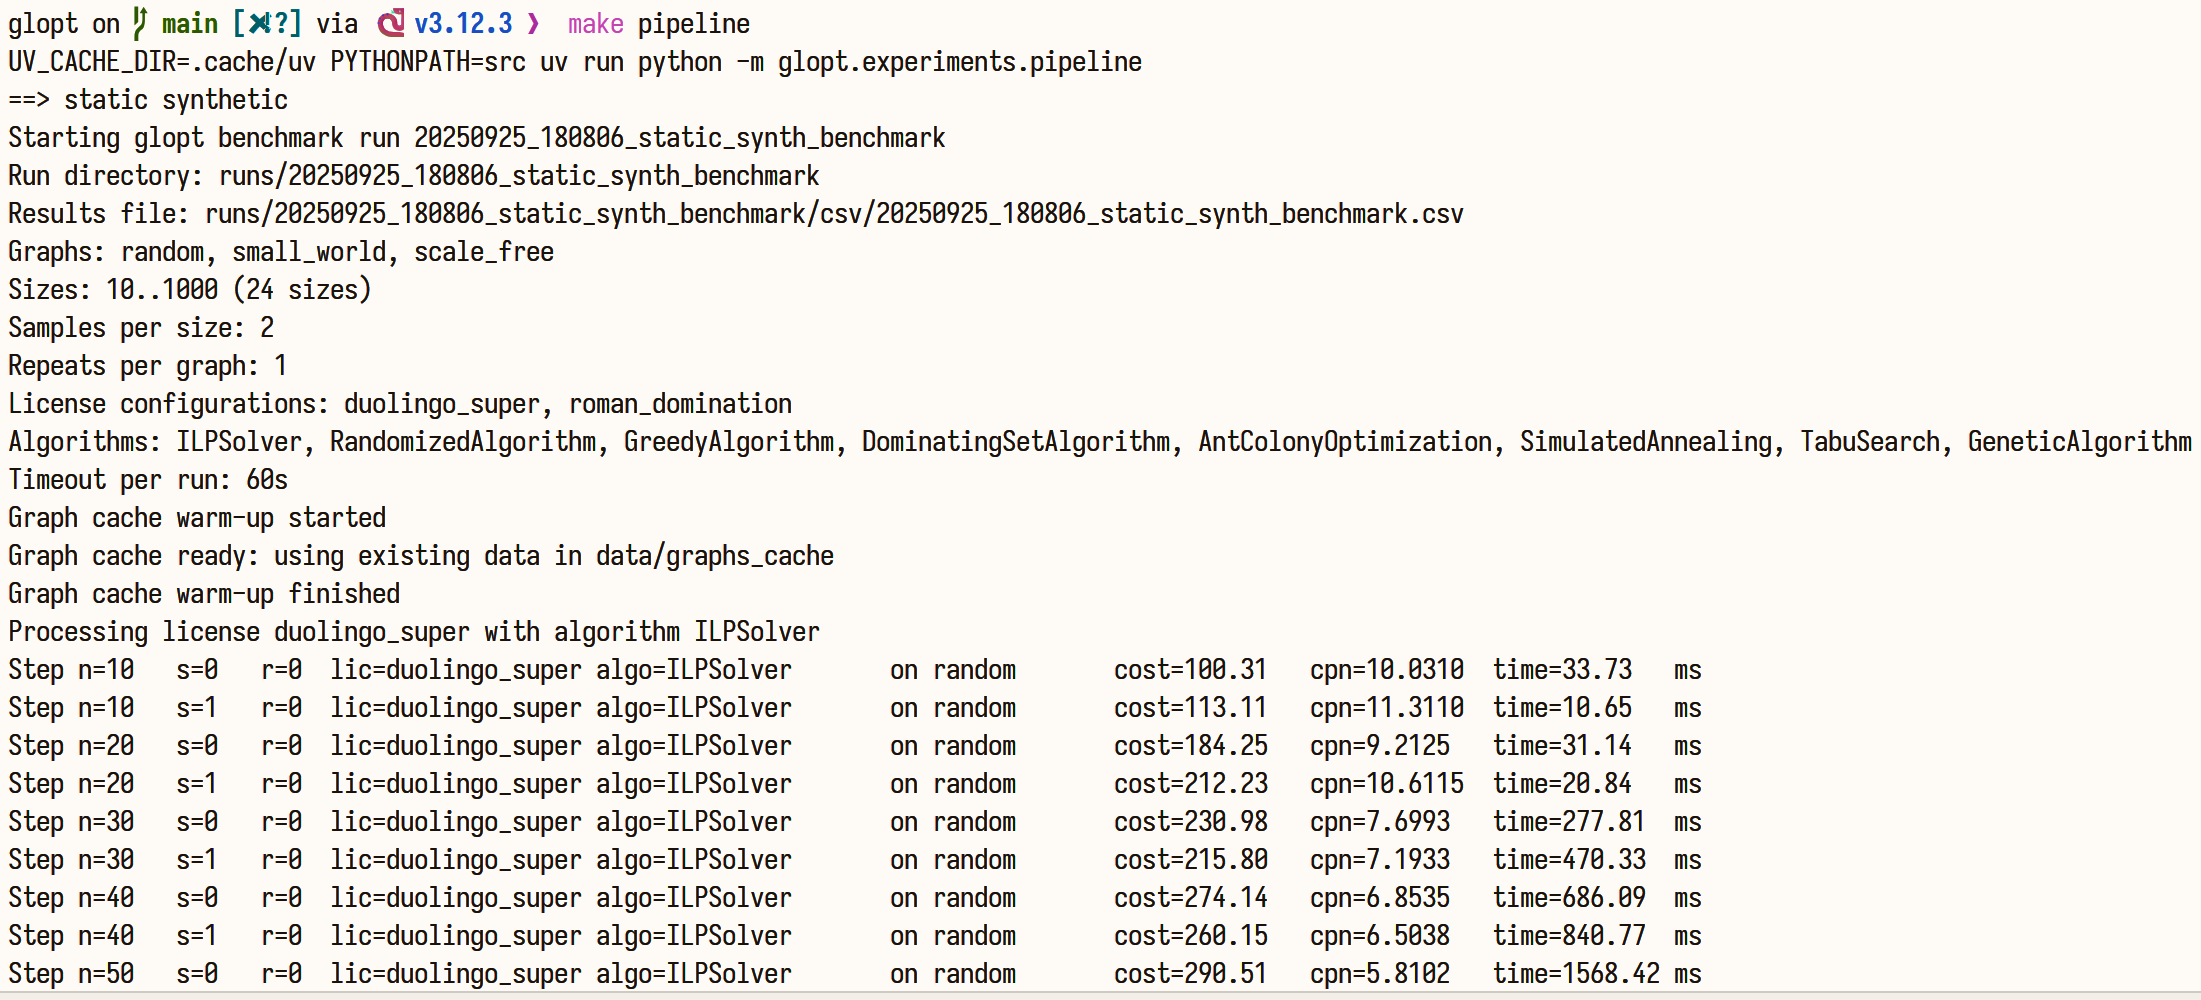
\includegraphics[width=0.95\linewidth]{assets/cli-content.png}
    \caption{Przykładowy przebieg uruchomienia potoku eksperymentalnego z Makefile.}
    \label{fig:cli-content}
\end{figure}

Na początku wyświetlane są informacje o wybranych parametrach uruchomienia, takich jak typ potoku, konfiguracje licencji, lista algorytmów oraz limity czasowe. Następnie rozpoczyna się proces przygotowania grafów. Tworzona jest pamięć podręczna grafów (cache), która umożliwia wielokrotne wykorzystanie tych samych instancji grafów między różnymi algorytmami i konfiguracjami licencji. Eliminuje to konieczność ponownego generowania grafów dla każdej próby, co istotnie skraca czas obliczeń, zwłaszcza dla dużych instancji.

Po przygotowaniu grafów wyświetlane są szczegóły dotyczące liczby rozmiarów, próbek i powtórzeń dla każdej instancji. Następnie dla każdej kombinacji licencji i algorytmu prezentowane są postępy obliczeń. Każda iteracja prezentuje podstawowe statystyki, takie jak rozmiar grafu, koszt rozwiązania, koszt na węzeł oraz czas wykonania. Umożliwia to bieżące monitorowanie przebiegu eksperymentu i szybkie wykrywanie ewentualnych anomalii.

\section{Organizacja skryptów eksperymentalnych}
Środowisko obliczeniowe zorganizowano jako spójny zestaw modułów
Pythona: pakiety do benchmarków statycznych, osobne moduły do
symulacji dynamicznych i rozszerzeń, a także proste komendy CLI do
szybkiej diagnostyki pojedynczych algorytmów. Wspólny rdzeń dba o
jednolite budowanie i walidację rozwiązań, a skrypty analityczne
tworzą raporty i wykresy użyte w częściach eksperymentalnych.

\section{Algorytmy dokładne}
\subsection{Program całkowitoliczbowy}
Pełna implementacja solvera ILP wykorzystującego bibliotekę PuLP
z solverem CBC do wyznaczania rozwiązań wzorcowych.

    {\footnotesize
        \begin{verbatim}
class ILPSolver(Algorithm):
    def solve(self, graph: nx.Graph, license_types: Sequence[LicenseType], **kwargs) -> Solution:
        # G = (V,E), N[i] = neighbors(i) union {i}
        nodes: list[Any] = list(graph.nodes())
        Nhood: dict[Any, set[Any]] = {i: set(graph.neighbors(i)) | {i} for i in nodes}
        degp1: dict[Any, int] = {i: len(Nhood[i]) for i in nodes}

        model = pulp.LpProblem("graph_licensing_optimization", pulp.LpMinimize)

        # active[i,t] = 1 gdy wlasciciel i otwiera grupe typu t
        active: dict[tuple[Any, int], pulp.LpVariable] = {}
        for i in nodes:
            for t_idx, lt in enumerate(license_types):
                feasible_owner_type = (lt.min_capacity <= degp1[i]) and (lt.max_capacity >= 1)
                if feasible_owner_type:
                    active[i, t_idx] = pulp.LpVariable(f"a_{i}_{t_idx}", cat="Binary")
                else:
                    # eliminacja niemozliwych par i,t
                    active[i, t_idx] = pulp.LpVariable(f"a_{i}_{t_idx}", lowBound=0, upBound=0, cat="Binary")

        # assign[i,j,t] = 1 gdy j nalezy do grupy wlasciciela i typu t
        assign: dict[tuple[Any, Any, int], pulp.LpVariable] = {}
        for i in nodes:
            for t_idx, lt in enumerate(license_types):
                if active[i, t_idx].upBound == 0:
                    continue
                if lt.max_capacity == 1:
                    # typ indywidualny, tylko wlasciciel
                    assign[i, i, t_idx] = pulp.LpVariable(f"x_{i}_{i}_{t_idx}", cat="Binary")
                else:
                    for j in Nhood[i]:
                        assign[i, j, t_idx] = pulp.LpVariable(f"x_{i}_{j}_{t_idx}", cat="Binary")

        # cel: min sum c_t * active[i,t]
        model += pulp.lpSum(active[i, t_idx] * license_types[t_idx].cost for i in nodes
                           for t_idx in range(len(license_types)))

        # co najwyzej jedna licencja na wlasciciela
        for i in nodes:
            model += pulp.lpSum(active[i, t_idx] for t_idx in range(len(license_types))) <= 1

        # pokrycie dokladnie raz
        for j in nodes:
            model += pulp.lpSum(assign.get((i, j, t_idx), 0) for i in Nhood[j]
                               for t_idx in range(len(license_types))) == 1

        # sprzezenie i pojemnosc
        for i in nodes:
            for t_idx, lt in enumerate(license_types):
                if active[i, t_idx].upBound == 0:
                    continue
                # wlasciciel nalezy do swojej grupy
                model += assign.get((i, i, t_idx), 0) == active[i, t_idx]
                # brak przypisan bez aktywacji
                for j in Nhood[i]:
                    var = assign.get((i, j, t_idx))
                    if var is not None:
                        model += var <= active[i, t_idx]
                # min i max pojemnosci tylko gdy aktywna
                group_size = pulp.lpSum(assign.get((i, j, t_idx), 0) for j in Nhood[i])
                model += group_size <= active[i, t_idx] * lt.max_capacity
                model += group_size >= active[i, t_idx] * lt.min_capacity

        # rozwiazanie ilp
        solver = pulp.PULP_CBC_CMD(msg=False)
        model.solve(solver)
        status = pulp.LpStatus.get(model.status, "Unknown")

        # fallback gdy brak rozwiazania dopuszczalnego
        if status in ("Infeasible", "Undefined", "Unbounded", "Not Solved"):
            singles = [lt for lt in license_types if lt.min_capacity <= 1 <= lt.max_capacity]
            if not singles:
                raise RuntimeError(f"ILP {status}: no single license available")
            lt = min(singles, key=lambda x: x.cost)
            groups = [LicenseGroup(license_type=lt, owner=i, additional_members=frozenset()) for i in nodes]
            return Solution(groups=tuple(groups))

        # ekstrakcja rozwiazania
        groups = []
        for i in nodes:
            for t_idx, lt in enumerate(license_types):
                a = active.get((i, t_idx))
                a_val = float(a.varValue) if a is not None and a.varValue is not None else 0.0
                if a_val > 0.5:
                    members: set[Any] = set()
                    for j in Nhood[i]:
                        var = assign.get((i, j, t_idx))
                        v_val = float(var.varValue) if var is not None and var.varValue is not None else 0.0
                        if v_val > 0.5:
                            members.add(j)
                    if members:
                        groups.append(
                            LicenseGroup(
                                license_type=lt,
                                owner=i,
                                additional_members=frozenset(members - {i}),
                            )
                        )

        return Solution(groups=tuple(groups))
\end{verbatim}
    }

\section{Algorytmy metaheurystyczne}
\subsection{Algorytm genetyczny}
Główne fragmenty implementacji algorytmu genetycznego z elityzmem,
selekcją turniejową oraz operatorami krzyżowania i mutacji.

    {\footnotesize
        \begin{verbatim}
class GeneticAlgorithm(Algorithm):
    def __init__(self, population_size: int = 30, num_generations: int = 40,
                 elite_fraction: float = 0.2, crossover_rate: float = 0.6):
        self.population_size = max(2, population_size)
        self.num_generations = max(1, num_generations)
        self.elite_fraction = max(0.0, min(1.0, elite_fraction))
        self.crossover_rate = max(0.0, min(1.0, crossover_rate))
        self.validator = SolutionValidator()

    def solve(self, graph: nx.Graph, license_types: Sequence[LicenseType], **kwargs) -> Solution:
        population = self._init_population(graph, license_types, initial)
        best = min(population, key=lambda s: s.total_cost)

        for _ in range(num_generations):
            population.sort(key=lambda s: s.total_cost)
            elite_count = max(1, int(self.elite_fraction * self.population_size))
            new_pop: list[Solution] = population[:elite_count]

            while len(new_pop) < self.population_size:
                if random.random() < self.crossover_rate and len(population) >= 2:
                    p1 = self._tournament_selection(population)
                    p2 = self._tournament_selection(population)
                    child = self._crossover(p1, p2, graph, license_types)
                    if not self.validator.is_valid_solution(child, graph):
                        base = min([p1, p2], key=lambda s: s.total_cost)
                        child = self._mutate(base, graph, license_types)
                else:
                    parent = self._tournament_selection(population)
                    child = self._mutate(parent, graph, license_types)
                new_pop.append(child)

            population = new_pop
            current_best = min(population, key=lambda s: s.total_cost)
            if current_best.total_cost < best.total_cost:
                best = current_best
        return best

    def _crossover(self, p1: Solution, p2: Solution, graph: nx.Graph,
                   license_types: Sequence[LicenseType]) -> Solution:
        def eff(g):
            return (g.license_type.cost / max(1, g.size), -g.size)

        candidates = list(p1.groups) + list(p2.groups)
        candidates.sort(key=eff)
        used = set()
        chosen: list = []
        for g in candidates:
            if used.isdisjoint(g.all_members):
                chosen.append(g)
                used.update(g.all_members)

        # Domknięcie niepokrytych węzłów algorytmem zachłannym
        uncovered = set(graph.nodes()) - used
        if uncovered:
            H = graph.subgraph(uncovered)
            filler = GreedyAlgorithm().solve(H, list(license_types))
            for fg in filler.groups:
                if set(fg.all_members).issubset(uncovered):
                    chosen.append(fg)

        child = SolutionBuilder.create_solution_from_groups(chosen)
        if not self.validator.is_valid_solution(child, graph):
            return GreedyAlgorithm().solve(graph, list(license_types))
        return child

    def _mutate(self, solution: Solution, graph: nx.Graph,
                license_types: Sequence[LicenseType]) -> Solution:
        neighbors = MutationOperators.generate_neighbors(solution, graph, license_types, k=5)
        valid_neighbors = [s for s in neighbors if self.validator.is_valid_solution(s, graph)]
        if not valid_neighbors:
            return solution
        return min(valid_neighbors, key=lambda s: s.total_cost)
\end{verbatim}
    }

\subsection{Optymalizacja mrówkowa}
Kluczowe fragmenty algorytmu mrówkowego z konstrukcją rozwiązań
oraz aktualizacją śladu feromonowego.

    {\footnotesize
        \begin{verbatim}
class AntColonyOptimization(Algorithm):
    def __init__(self, alpha: float = 1.0, beta: float = 2.0, evaporation: float = 0.5,
                 q0: float = 0.9, num_ants: int = 20):
        self.alpha, self.beta, self.evap, self.q0, self.num_ants = alpha, beta, evaporation, q0, num_ants

    def solve(self, graph: nx.Graph, license_types: Sequence[LicenseType], **kwargs) -> Solution:
        pher = self._init_pher(graph, license_types)  # Inicjalizacja feromonu
        heur = self._init_heur(graph, license_types)  # Informacja heurystyczna
        best = GreedyAlgorithm().solve(graph, license_types)
        self._deposit(pher, best)

        for _ in range(max_iter_aco):
            improved = False
            for _ in range(num_ants):
                cand = self._construct(graph, license_types, pher, heur)
                ok, _ = self.validator.validate(cand, graph)
                if ok and cand.total_cost < best.total_cost:
                    best, improved = cand, True
            self._evaporate(pher)
            self._deposit(pher, best)
        return best

    def _construct(self, graph: nx.Graph, lts: Sequence[LicenseType],
                   pher: dict, heur: dict) -> Solution:
        uncovered: set[Any] = set(graph.nodes())
        groups: list[LicenseGroup] = []

        while uncovered:
            owner = self._select_owner(uncovered, lts, pher, heur)
            lt = self._select_license(owner, lts, pher, heur)

            pool = (set(graph.neighbors(owner)) | {owner}) & uncovered
            if len(pool) < lt.min_capacity:
                # Fallback do licencji indywidualnej
                singles = [x for x in lts if x.min_capacity <= 1 <= x.max_capacity]
                lt = min(singles, key=lambda x: x.cost) if singles else lt
                groups.append(LicenseGroup(lt, owner, frozenset()))
                uncovered.remove(owner)
                continue

            # Wybór członków grupy według stopnia
            k = max(0, lt.max_capacity - 1)
            add = sorted((pool - {owner}), key=lambda n: graph.degree[n], reverse=True)[:k]
            groups.append(LicenseGroup(lt, owner, frozenset(add)))
            uncovered -= {owner} | set(add)

        return Solution(groups=tuple(groups))

    def _select_owner(self, uncovered: set, lts: Sequence[LicenseType],
                      pher: dict, heur: dict) -> Any:
        scores = {}
        for n in uncovered:
            acc = sum((pher.get((n, lt.name), 1.0) ** self.alpha) *
                     (heur.get((n, lt.name), 1.0) ** self.beta) for lt in lts)
            scores[n] = acc / max(1, len(lts))
        return self._roulette_or_best(list(uncovered), scores)

    def _evaporate(self, pher: dict) -> None:
        for k in pher:
            pher[k] *= (1.0 - self.evap)

    def _deposit(self, pher: dict, sol: Solution) -> None:
        if sol.total_cost > 0:
            q = 1.0 / sol.total_cost
            for g in sol.groups:
                for n in g.all_members:
                    k = (n, g.license_type.name)
                    if k in pher:
                        pher[k] += q
\end{verbatim}
    }

\subsection{Wyżarzanie symulowane}
Fragment implementacji wyżarzania z generowaniem sąsiadów
i akceptacją według kryterium Metropolisa.

    {\footnotesize
        \begin{verbatim}
class SimulatedAnnealing(Algorithm):
    def solve(self, graph: nx.Graph, license_types: Sequence[LicenseType], **kwargs) -> Solution:
        current = GreedyAlgorithm().solve(graph, license_types)
        best = current
        temp = self.temp_initial
        stall = 0

        for _ in range(self.max_iterations):
            if temp < self.temp_min:
                break

            cand = self._neighbor(current, graph, license_types)
            if cand is None:
                stall += 1
            else:
                delta = cand.total_cost - current.total_cost
                if delta < 0 or random.random() < math.exp(-delta / max(temp, 1e-10)):
                    current = cand
                    if current.total_cost < best.total_cost:
                        best, stall = current, 0
                    else:
                        stall += 1
                else:
                    stall += 1

            if stall >= self.max_stall:
                stall, temp = 0, max(self.temp_min, 0.5 * temp)
            temp *= self.cooling_rate

        return best

    def _neighbor(self, solution: Solution, graph: nx.Graph, lts: Sequence[LicenseType]) -> Solution:
        moves = [self._mv_change_license, self._mv_move_member,
                 self._mv_swap_members, self._mv_merge_groups, self._mv_split_group]

        for _ in range(12):
            mv = random.choice(moves)
            try:
                cand = mv(solution, graph, lts)
                if cand and self.validator.validate(cand, graph)[0]:
                    return cand
            except Exception:
                continue
        return None
\end{verbatim}
    }

\section{Operatory mutacji i sąsiedztwa}
Kluczowe operatory używane przez metaheurystyki do generowania
sąsiadów i eksploracji przestrzeni rozwiązań.

{\footnotesize
\begin{verbatim}
class MutationOperators:
    @staticmethod
    def generate_neighbors(base: Solution, graph: nx.Graph,
                          license_types: Sequence[LicenseType], k: int = 10) -> list[Solution]:
        ops = (MutationOperators.change_license_type, MutationOperators.reassign_member,
               MutationOperators.merge_groups, MutationOperators.split_group)
        weights = (0.3, 0.3, 0.2, 0.2)
        out: list[Solution] = []
        attempts = 0

        while len(out) < k and attempts < k * 10:
            attempts += 1
            op = random.choices(ops, weights=weights, k=1)[0]
            try:
                cand = op(base, graph, list(license_types))
                if cand is not None:
                    out.append(cand)
            except Exception:
                continue
        return out

    @staticmethod
    def change_license_type(solution: Solution, graph: nx.Graph,
                           license_types: list[LicenseType]) -> Solution | None:
        if not solution.groups:
            return None
        group = random.choice(solution.groups)
        compatible = SolutionBuilder.get_compatible_license_types(
            group.size, license_types, exclude=group.license_type
        )
        if not compatible:
            return None

        new_lt = random.choice(compatible)
        new_groups = []
        for g in solution.groups:
            if g is group:
                new_groups.append(LicenseGroup(new_lt, g.owner, g.additional_members))
            else:
                new_groups.append(g)
        return SolutionBuilder.create_solution_from_groups(new_groups)

    @staticmethod
    def reassign_member(solution: Solution, graph: nx.Graph,
                       license_types: list[LicenseType]) -> Solution | None:
        if len(solution.groups) < 2:
            return None

        donors = [g for g in solution.groups
                 if g.size > g.license_type.min_capacity and g.additional_members]
        receivers = [g for g in solution.groups if g.size < g.license_type.max_capacity]

        if not donors or not receivers:
            return None

        from_group = random.choice(donors)
        pot_receivers = [g for g in receivers if g is not from_group]
        if not pot_receivers:
            return None

        to_group = random.choice(pot_receivers)
        member = random.choice(list(from_group.additional_members))
        allowed = SolutionBuilder.get_owner_neighbors_with_self(graph, to_group.owner)

        if member not in allowed:
            return None

        # Przeprowadzenie transferu
        new_groups = []
        for g in solution.groups:
            if g is from_group:
                new_groups.append(LicenseGroup(
                    g.license_type, g.owner, g.additional_members - {member}
                ))
            elif g is to_group:
                new_groups.append(LicenseGroup(
                    g.license_type, g.owner, g.additional_members | {member}
                ))
            else:
                new_groups.append(g)

        return SolutionBuilder.create_solution_from_groups(new_groups)

    @staticmethod
    def split_group(solution: Solution, graph: nx.Graph,
                   license_types: list[LicenseType]) -> Solution | None:
        splittable = [g for g in solution.groups if g.size > 2]
        if not splittable:
            return None

        group = random.choice(splittable)
        members = list(group.all_members)

        for _ in range(4):  # Próbuj kilka podziałów
            random.shuffle(members)
            cut = random.randint(1, len(members) - 1)
            part1, part2 = members[:cut], members[cut:]

            # Sprawdź kompatybilność typów licencji
            compat1 = SolutionBuilder.get_compatible_license_types(len(part1), license_types)
            compat2 = SolutionBuilder.get_compatible_license_types(len(part2), license_types)

            if not compat1 or not compat2:
                continue

            # Wybierz właścicieli i typy licencji
            owner1, owner2 = random.choice(part1), random.choice(part2)
            lt1, lt2 = min(compat1, key=lambda x: x.cost), min(compat2, key=lambda x: x.cost)

            # Sprawdź ograniczenia sąsiedztwa
            if (set(part1).issubset(SolutionBuilder.get_owner_neighbors_with_self(graph, owner1)) and
                set(part2).issubset(SolutionBuilder.get_owner_neighbors_with_self(graph, owner2))):

                new_groups = [g for g in solution.groups if g is not group]
                new_groups.append(LicenseGroup(lt1, owner1, frozenset(set(part1) - {owner1})))
                new_groups.append(LicenseGroup(lt2, owner2, frozenset(set(part2) - {owner2})))
                return SolutionBuilder.create_solution_from_groups(new_groups)

        return None
\end{verbatim}
}

\section{Funkcje pomocnicze}
\subsection{Budowanie i walidacja rozwiązań}
Klasy pomocnicze odpowiedzialne za tworzenie i weryfikację poprawności rozwiązań.

{\footnotesize
\begin{verbatim}
class SolutionBuilder:
    @staticmethod
    def get_compatible_license_types(group_size: int, license_types: Sequence[LicenseType],
                                   exclude: LicenseType | None = None) -> list[LicenseType]:
        out: list[LicenseType] = []
        for lt in license_types:
            if exclude and lt == exclude:
                continue
            if lt.min_capacity <= group_size <= lt.max_capacity:
                out.append(lt)
        return out

    @staticmethod
    def get_owner_neighbors_with_self(graph: nx.Graph, owner: N) -> set[N]:
        return set(graph.neighbors(owner)) | {owner}

    @staticmethod
    def find_cheapest_single_license(license_types: Sequence[LicenseType]) -> LicenseType:
        singles = [lt for lt in license_types if lt.min_capacity <= 1]
        return min(singles or list(license_types), key=lambda lt: lt.cost)

class SolutionValidator:
    def validate(self, solution: Solution[N], graph: nx.Graph) -> tuple[bool, list[ValidationIssue]]:
        issues: list[ValidationIssue] = []
        nodes = set(graph.nodes())
        groups = tuple(solution.groups)

        # Sprawdzanie członków grup
        issues += self._check_group_members(groups, nodes)
        # Sprawdzanie pojemności licencji
        issues += self._check_group_capacity(groups)
        # Sprawdzanie ograniczeń sąsiedztwa
        issues += self._check_neighbors(groups, graph, nodes)
        # Sprawdzanie braku nakładania się grup
        issues += self._check_no_overlap(groups)
        # Sprawdzanie pokrycia wszystkich węzłów
        issues += self._check_coverage(groups, nodes)

        return (not issues, issues)

    def _check_neighbors(self, groups: tuple[LicenseGroup[N], ...], graph: nx.Graph,
                        nodes: set[N]) -> list[ValidationIssue]:
        issues: list[ValidationIssue] = []
        for idx, g in enumerate(groups):
            if g.owner not in nodes:
                continue
            allowed_any = set(graph.neighbors(g.owner)) | {g.owner}
            not_neighbors = set(g.all_members) - allowed_any
            if not_neighbors:
                issues.append(ValidationIssue(
                    "DISCONNECTED_MEMBER",
                    f"group#{idx} owner {g.owner!r} has non-neighbor members: {list(not_neighbors)!r}"
                ))
        return issues

    def _check_coverage(self, groups: tuple[LicenseGroup[N], ...], nodes: set[N]) -> list[ValidationIssue]:
        issues: list[ValidationIssue] = []
        covered = set().union(*(set(g.all_members) for g in groups)) if groups else set()
        missing = nodes - covered
        if missing:
            issues.append(ValidationIssue("MISSING_COVERAGE", f"missing nodes: {list(missing)!r}"))
        return issues
\end{verbatim}
}

\subsection{Konfiguracje licencyjne}
Fabryka konfiguracji licencyjnych obsługująca różne rodziny
licencji oraz dynamiczne warianty cenowe.

    {\footnotesize
        \begin{verbatim}
class LicenseConfigFactory:
    _CONFIGS: ClassVar[dict[str, Callable[[], list[LicenseType]]]] = {
        "duolingo_super": lambda: [
            LicenseType("Individual", 13.99, 1, 1, LicenseConfigFactory.BLACK),
            LicenseType("Family", 29.17, 2, 6, LicenseConfigFactory.BLACK),
        ],
        "spotify": lambda: [
            LicenseType("Individual", 23.99, 1, 1, LicenseConfigFactory.RED),
            LicenseType("Duo", 30.99, 2, 2, LicenseConfigFactory.GREEN),
            LicenseType("Family", 37.99, 2, 6, LicenseConfigFactory.BLUE),
        ],
        "netflix": lambda: [
            LicenseType("Basic", 33, 1, 1, LicenseConfigFactory.RED),
            LicenseType("Standard", 49, 1, 2, LicenseConfigFactory.GREEN),
            LicenseType("Premium", 67, 1, 4, LicenseConfigFactory.BLUE),
        ],
        "roman_domination": lambda: [
            LicenseType("Solo", 1.0, 1, 1, LicenseConfigFactory.BLUE),
            LicenseType("Group", 2.0, 2, 999999, LicenseConfigFactory.RED),
        ],
    }

    @classmethod
    def get_config(cls, name: str) -> list[LicenseType]:
        # Obsługa dynamicznych wariantów roman_p_<price>
        if name.startswith("roman_p_"):
            p_str = name.split("_", 2)[2].replace("_", ".")
            try:
                p_val = float(p_str)
                return [
                    LicenseType("Solo", 1.0, 1, 1, cls.BLUE),
                    LicenseType("Group", p_val, 2, 999999, cls.RED),
                ]
            except Exception:
                raise ValueError(f"Invalid roman price format: {name}")

        # Obsługa dynamicznych wariantów duolingo_p_<price>
        if name.startswith("duolingo_p_"):
            p_str = name.split("_", 2)[2].replace("_", ".")
            try:
                p_val = float(p_str)
                return [
                    LicenseType("Individual", 1.0, 1, 1, cls.RED),
                    LicenseType("Family", p_val, 2, 6, cls.BLUE),
                ]
            except Exception:
                raise ValueError(f"Invalid duolingo price format: {name}")

        # Konfiguracje statyczne
        try:
            return cls._CONFIGS[name]()
        except KeyError:
            available = ", ".join(cls._CONFIGS.keys())
            raise ValueError(f"Unsupported license config: {name}. Available: {available}")
\end{verbatim}
    }

\section{Symulacja dynamiczna}
\subsection{Symulator ewolucji sieci}
Główne komponenty symulatora odpowiedzialnego za mutacje
struktury grafu w eksperymentach dynamicznych.

    {\footnotesize
        \begin{verbatim}
@dataclass
class MutationParams:
    add_nodes_prob: float = 0.1
    remove_nodes_prob: float = 0.05
    add_edges_prob: float = 0.15
    remove_edges_prob: float = 0.1
    max_nodes_add: int = 3
    max_nodes_remove: int = 2
    max_edges_add: int = 5
    max_edges_remove: int = 3
    mode_nodes: str = "random"      # "random" lub "preferential"
    mode_edges: str = "random"      # "random", "preferential", "triadic", "rewire_ws"
    add_node_attach_m: int = 2
    triadic_trials: int = 20

class DynamicNetworkSimulator:
    def __init__(self, mutation_params: MutationParams | None = None, seed: int | None = None):
        self.mutation_params = mutation_params or MutationParams()
        self.next_node_id = 0
        if seed is not None:
            random.seed(seed)

    def _apply_mutations(self, graph: nx.Graph) -> tuple[nx.Graph, list[str]]:
        mutations = []

        # Dodawanie węzłów
        if random.random() < self.mutation_params.add_nodes_prob:
            num_add = random.randint(1, self.mutation_params.max_nodes_add)
            new_nodes = self._add_nodes(graph, num_add)
            mutations.append(f"Added nodes: {new_nodes}")

        # Usuwanie węzłów (z zachowaniem minimalnego rozmiaru)
        if (random.random() < self.mutation_params.remove_nodes_prob
            and graph.number_of_nodes() > 5):
            num_remove = random.randint(1, min(self.mutation_params.max_nodes_remove,
                                              graph.number_of_nodes() - 5))
            removed_nodes = self._remove_nodes(graph, num_remove)
            mutations.append(f"Removed nodes: {removed_nodes}")

        # Dodawanie krawędzi
        if random.random() < self.mutation_params.add_edges_prob:
            num_add = random.randint(1, self.mutation_params.max_edges_add)
            if self.mutation_params.mode_edges == "rewire_ws":
                added_c, removed_c = self._rewire_edges(graph, num_add)
                if added_c: mutations.append(f"Added {added_c} edges")
                if removed_c: mutations.append(f"Removed {removed_c} edges")
            else:
                added_edges = self._add_edges(graph, num_add)
                mutations.append(f"Added {len(added_edges)} edges")

        return (graph, mutations)

    def _add_nodes(self, graph: nx.Graph, num_nodes: int) -> list[int]:
        new_nodes = []
        existing_nodes = list(graph.nodes())

        for _ in range(num_nodes):
            new_node = self.next_node_id
            self.next_node_id += 1
            graph.add_node(new_node)
            new_nodes.append(new_node)

            # Podłączanie do istniejących węzłów
            if existing_nodes:
                m = min(self.mutation_params.add_node_attach_m, len(existing_nodes))

                if self.mutation_params.mode_nodes == "preferential":
                    # Attachment proporcjonalny do stopni węzłów
                    deg = graph.degree
                    weights = [deg[v] + 1 for v in existing_nodes]
                    total = sum(weights)
                    chosen = set()

                    for _ in range(m):
                        if not existing_nodes: break
                        r = random.uniform(0, total)
                        acc, pick_idx = 0.0, 0
                        for idx, w in enumerate(weights):
                            acc += w
                            if acc >= r:
                                pick_idx = idx
                                break
                        v = existing_nodes[pick_idx]
                        if v not in chosen:
                            graph.add_edge(new_node, v)
                            chosen.add(v)
                        total -= weights[pick_idx]
                        existing_nodes.pop(pick_idx)
                        weights.pop(pick_idx)
                else:
                    # Losowe podłączanie
                    neighbors = random.sample(existing_nodes, m)
                    for neighbor in neighbors:
                        graph.add_edge(new_node, neighbor)

            existing_nodes = list(graph.nodes())

        return new_nodes

    def _add_edges(self, graph: nx.Graph, num_edges: int) -> list[tuple[int, int]]:
        nodes = list(graph.nodes())
        added_edges = []
        if len(nodes) < 2: return added_edges

        mode = self.mutation_params.mode_edges
        if mode == "triadic":
            # Zamykanie trójkątów
            attempts = 0
            while len(added_edges) < num_edges and attempts < num_edges * 20:
                w = random.choice(nodes)
                neigh = list(graph.neighbors(w))
                if len(neigh) >= 2:
                    u, v = random.sample(neigh, 2)
                    if not graph.has_edge(u, v):
                        graph.add_edge(u, v)
                        added_edges.append((u, v))
                attempts += 1

        elif mode == "preferential":
            # Preferencyjne dodawanie proporcjonalne do iloczynów stopni
            attempts = 0
            while len(added_edges) < num_edges and attempts < num_edges * 20:
                u, v = random.sample(nodes, 2)
                if graph.has_edge(u, v):
                    attempts += 1
                    continue
                deg = graph.degree
                w = (deg[u] + 1) * (deg[v] + 1)
                max_deg = max((deg[x] for x in nodes), default=1)
                accept_p = min(1.0, w / float((max_deg + 1) ** 2))
                if random.random() < accept_p:
                    graph.add_edge(u, v)
                    added_edges.append((u, v))
                attempts += 1

        return added_edges
\end{verbatim}
    }
